\documentclass{standalone}
\usepackage{times}
\usepackage{mathtools}
\usepackage{amsfonts}
\usepackage{amssymb}

\usepackage{tikz}
\usetikzlibrary{positioning,fit,shapes,calc,decorations.pathreplacing}
\usetikzlibrary{backgrounds}
\usetikzlibrary{arrows.meta}
\usetikzlibrary{shapes,snakes}

\definecolor{processblue}{cmyk}{1,1,1,0}
\definecolor{accent}{rgb}{0.0,0.5,0.8}
\definecolor{accent2}{rgb}{0.8,0.5,0.0}

\begin{document}
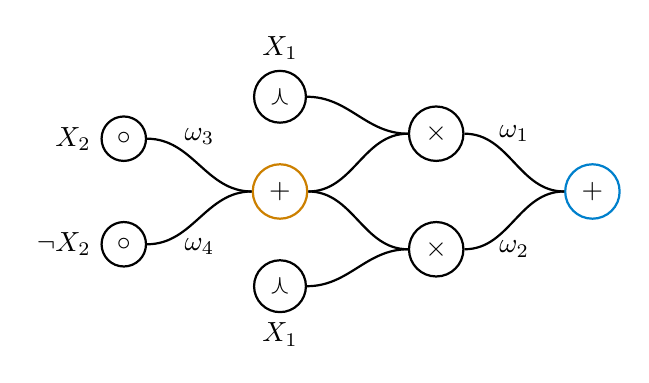
\begin{tikzpicture}[
  node/.style = {
    draw,
    circle,
    thick,
    fill = white,
    minimum width = 0.5cm,
    minimum height = 0.5cm,
  },
  >={Stealth[scale=1.8]},
]

  \node[node,draw=accent2] (a) {$+$};

  \node (left) [left=1.5cm of a] {};
  \node (right) [right=1.5cm of a] {};
  \node[node,draw=accent] (root) [right=1.5cm of right] {$+$};

  \node[node] (b) [above=0.25cm of left,label={left:$X_2$}] {$\circ$};
  \node[node] (c) [below=0.25cm of left,label={left:$\lnot X_2$}] {$\circ$};

  \node[node] (d) [above=0.25cm of right] {$\times$};
  \node[node] (e) [below=0.25cm of right] {$\times$};

  \node[node] (f) [above=0.5cm of a,label={above:$X_1$}] {$\curlywedge$};
  \node[node] (g) [below=0.5cm of a,label={below:$X_1$}] {$\curlywedge$};


  \path[-,thick] (b) edge[out=0,in=180] node [label={above:$\omega_3$}] {} (a);
  \path[-,thick] (c) edge[out=0,in=180] node [label={below:$\omega_4$}] {} (a);

  \path[-,thick] (a) edge[out=0,in=180] node {} (d);
  \path[-,thick] (a) edge[out=0,in=180] node {} (e);

  \path[-,thick] (f) edge[out=0,in=180] node {} (d);
  \path[-,thick] (g) edge[out=0,in=180] node {} (e);

  \path[-,thick] (d) edge[out=0,in=180] node [label={above:$\omega_1$}] {} (root);
  \path[-,thick] (e) edge[out=0,in=180] node [label={below:$\omega_2$}] {} (root);

\end{tikzpicture}
\end{document}
